\chapter{Anomaly Detection}
\label{ch:anomaly}

\section{Methods}

Two anomaly detection methods are implemented and compared:

\subsection{Statistical Thresholds}

For each hour of the day (0--23), the mean $\mu_h$ and standard deviation $\sigma_h$ of load power are computed from training data. A measurement at hour $h$ is flagged as anomalous if:

\begin{equation}
    P_{\text{load}}(t) > \mu_h + k \cdot \sigma_h \quad \text{or} \quad P_{\text{load}}(t) < \mu_h - k \cdot \sigma_h
\end{equation}

with $k = 2.5$.

\subsection{Isolation Forest}

An Isolation Forest model is trained on 8 features: load power, hour, day of week, weekend flag, temperature, irradiance, PV power, and SOC. The contamination parameter is set to 0.02 (assuming 2\% of training data may contain anomalies).

\section{Results}

\begin{figure}[H]
    \centering
    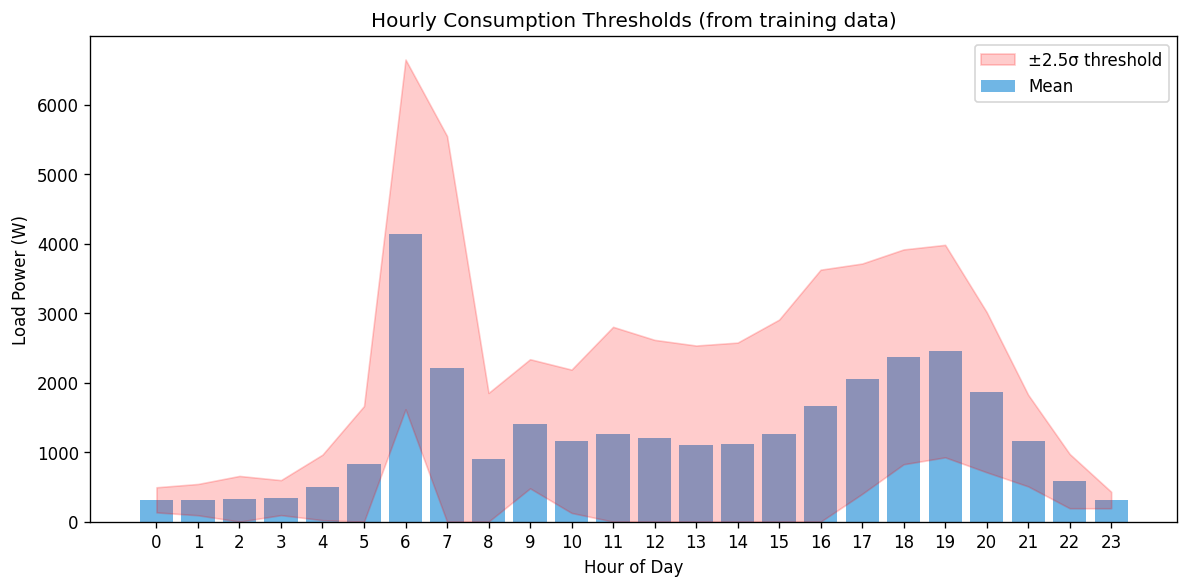
\includegraphics[width=0.85\textwidth]{figures/anomaly_thresholds.png}
    \caption{Per-hour consumption thresholds computed from training data ($k=2.5$).}
    \label{fig:anomaly_thresholds}
\end{figure}

Table~\ref{tab:anomaly_results} compares both methods against the ground-truth anomaly labels injected during simulation.

\begin{table}[H]
\centering
\caption{Anomaly detection comparison on the detection set.}
\label{tab:anomaly_results}
\begin{tabular}{lrrrr}
\toprule
\textbf{Method} & \textbf{Precision} & \textbf{Recall} & \textbf{F1} & \textbf{TP / FP} \\
\midrule
Statistical ($k=2.5$) & 0.085 & 0.710 & 0.151 & 44 / 475 \\
Isolation Forest & 0.016 & 0.097 & 0.027 & 6 / 374 \\
\bottomrule
\end{tabular}
\end{table}

\section{Discussion}

\begin{figure}[H]
    \centering
    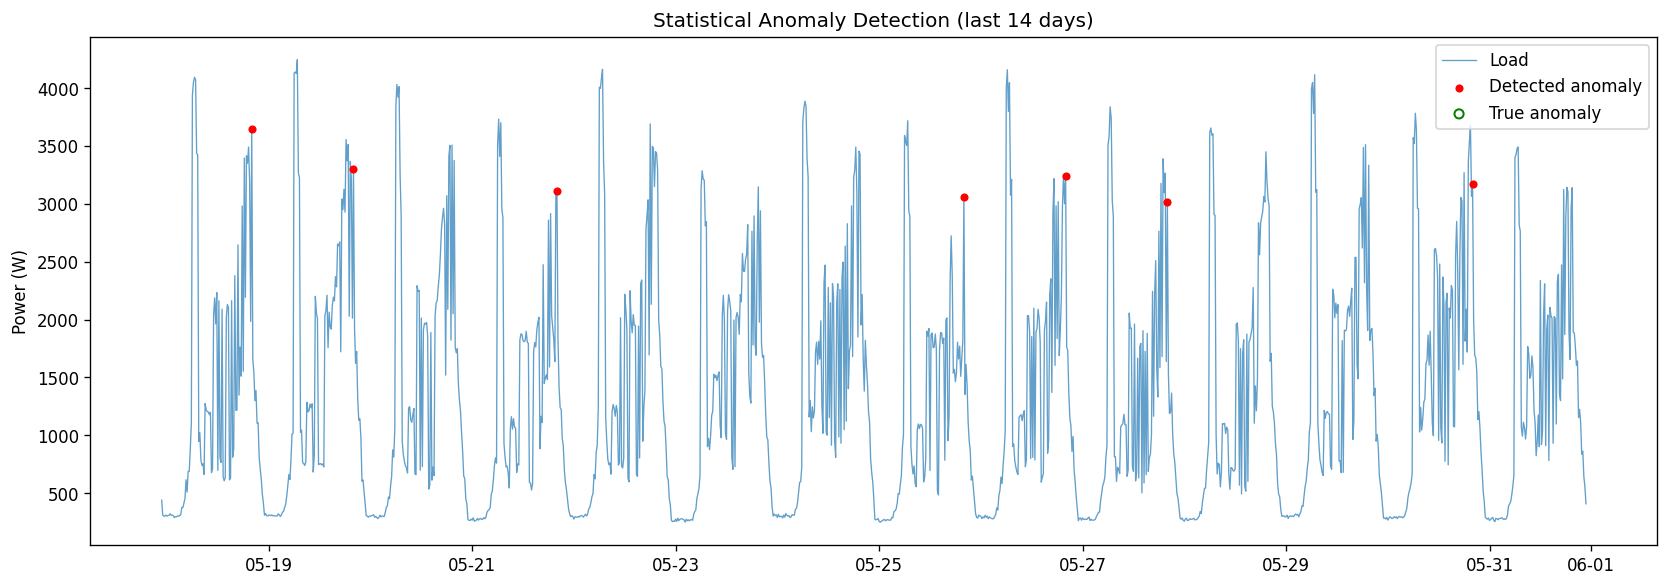
\includegraphics[width=\textwidth]{figures/anomaly_statistical.png}
    \caption{Statistical anomaly detection results (last 14 days). Red dots: detected anomalies; green circles: ground-truth anomalies.}
    \label{fig:anomaly_stat}
\end{figure}

\begin{figure}[H]
    \centering
    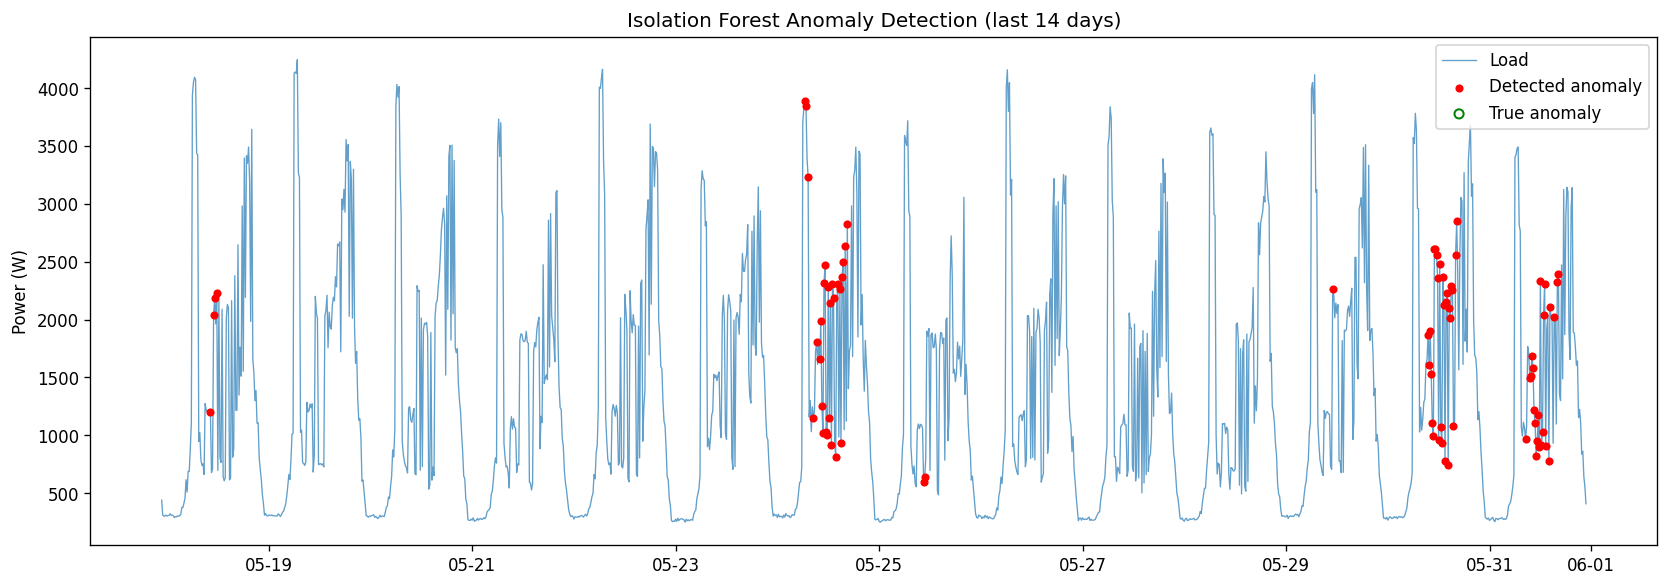
\includegraphics[width=\textwidth]{figures/anomaly_iforest.png}
    \caption{Isolation Forest anomaly detection results (last 14 days).}
    \label{fig:anomaly_if}
\end{figure}

The statistical method achieves significantly higher recall (71\%) than Isolation Forest (10\%), detecting most of the injected anomalies. However, precision is low (8.5\%) because the building's natural load variability (AC compressor cycling, flexible loads) creates many false positives above the $\mu + 2.5\sigma$ threshold.

The Isolation Forest performs poorly because the injected anomalies (load spikes) overlap with normal high-load patterns in the 8-dimensional feature space. This method would likely perform better with real data where anomalies have more distinctive signatures.

For a production system, the statistical method is recommended with:
\begin{itemize}[nosep]
    \item Increased $k$ (e.g., 3.0--3.5) to reduce false positives.
    \item Contextual filtering (suppress alerts during known high-load periods).
    \item Separate thresholds for weekday vs.\ weekend patterns.
\end{itemize}

\section{Alert Generation}

Detected anomalies are classified by type (night consumption, high load, PV drop) and severity (info, warning, critical), and stored in the alerts database table. The dashboard provides filtering, acknowledgment, and timeline visualization.
